\vspace{-30pt}
\begin{figure*}[h!]
    \centering
    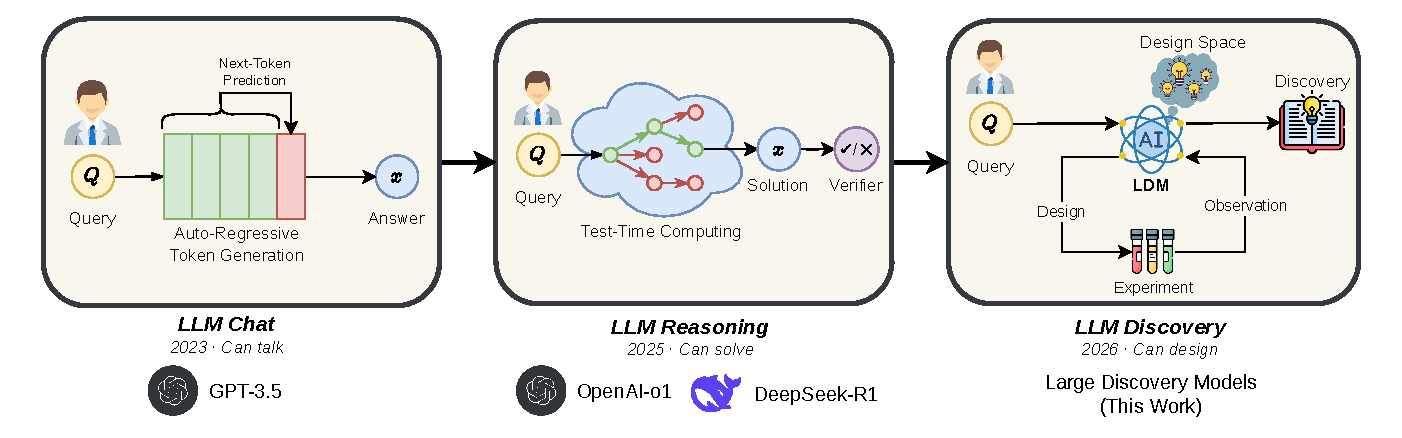
\includegraphics[width=\textwidth]{figure/evolution.drawio.pdf}
    \vspace{-20pt}
    \caption{
    \textbf{From generation and reasoning to open-ended discovery.}
    \emph{LLM generation} produces a response to a user query through
    autoregressive prediction \citep{brownLanguageModelsAre2020}.
    \emph{LLM reasoning} uses additional inference-time computation, such as
    chain-of-thought, tree search, or best-of-$N$ sampling, to generate,
    evaluate, and refine candidate solutions, typically with access to a cheap verifier \citep{openaiOpenAIO1System2024,wang2024openr,
    deepseek-aiDeepSeekR1IncentivizingReasoning2025}.
    \emph{Large Discovery Models} extend this loop to open-ended scientific
    design spaces, where evaluation requires costly interaction with the
    external world. Experimental observations update the model and guide the
    subsequent generation and selection of hypotheses or designs.
    }
    \label{fig:evolution}
\end{figure*}


\section{Introduction}
\label{sec:intro}

The development of large language models (LLMs) has progressed from
open-ended generation towards increasingly capable forms of reasoning.
Pretraining provides broad linguistic and conceptual knowledge, while
inference-time scaling allows a model to generate, compare, and refine
multiple candidate solutions. This approach has produced substantial gains in
mathematics, coding, theorem proving, and game playing, where solutions may be
difficult to find but comparatively easy to evaluate. Formal derivations can
be assessed by process or outcome verifiers, programs can be executed against
unit tests, and game strategies can be evaluated using exact rules or
simulators
\citep{yao2023tree,madaan2023selfrefine,snell2025scaling}.
AlphaZero-like methods make this feedback loop explicit by combining
generation, evaluation, and search
\citep{silver2017mastering,fengAlphazerolikeTreeSearchCan2024}.
OpenR~\citep{wang2024openr} provides an open framework for studying such
reasoning systems, while AlphaEvolve~\citep{novikov2025alphaevolve} couples
language-model proposals with automated evaluators at scale. Together, these
developments demonstrate that inference-time computation is particularly
effective when reliable and repeatable feedback can turn generation into
directed search.

Scientific discovery poses a more challenging setting. The candidate space may be vast, structured, and only partially specified, while feedback often depends on expensive simulation, accelerator experiments, physical assays, or real-world experiment. Evaluations cannot be repeated freely, and the resulting feedback may be delayed or noisy. A discovery system must therefore decide not only which candidates to evaluate, but also which hypotheses and designs should enter the search process in the first place. Figure~\ref{fig:evolution} illustrates this progression from generation and reasoning to discovery.



\begin{definition}[Scientific discovery]
\label{def:scientific-discovery}
Scientific discovery, in the setting considered here, is a sequential process
in which an agent generates hypotheses or designs, selects a limited number
for evaluation through interaction with an external evaluator, and uses the
resulting empirical observations to update its beliefs and guide subsequent
search. A discovery occurs when this
process identifies a previously unknown and non-trivial relationship,
mechanism, or design that is supported by empirical evidence.\footnote{This is an operational definition of empirically grounded,
search-based scientific discovery: the class of scientific problems that can
be formulated as sequential search over hypotheses or designs, with selected
candidates evaluated through physical experiments, simulations, computational
tests, or other external sources of evidence. It does not encompass all forms
of scientific discovery, particularly those for which the relevant search
space, evaluation procedure, or objective cannot yet be specified. Moreover,
\emph{unknown} and \emph{non-trivial} are relational notions, defined relative
to the agent's prior knowledge and, where appropriate, the knowledge of the
relevant scientific community. A result may therefore be a discovery for an
agent while constituting a rediscovery from the community's perspective.}
\end{definition}

\begin{figure*}[h]
    \centering
    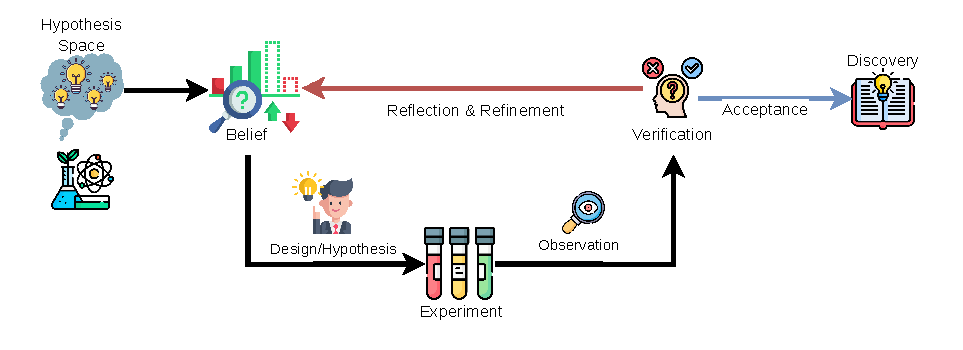
\includegraphics[width=\textwidth]
    {figure/discovery.drawio.pdf}
    \caption{
    \textbf{The Experimental Scientific Discovery (ESD) loop.}
    An agent generates candidate hypotheses or designs, selects a subset for
    costly evaluation, observes the outcomes, and uses those observations to
    update its beliefs and guide the next round of search, as described in
    Definition~\ref{def:scientific-discovery}.
    }
    \label{fig:scientific-discovery}
\end{figure*}

Definition~\ref{def:scientific-discovery} highlights two differences between
scientific discovery and reasoning with cheap verifiers. First, scientific
search is often \emph{open-ended}: relevant candidates may lie outside the
region represented by the current model or reachable through its existing
search operators. Second, empirical feedback is \emph{budgeted}: only a small
fraction of the generated candidates can be evaluated. The agent must
therefore learn from limited observations, model an unknown objective, and
allocate its experimental budget to candidates that are expected to be useful
or informative
\citep{shahriari2016taking,frazier2018tutorial}.

Current LLM-based research systems address only part of this problem.
Autonomous research agents can generate hypotheses, write code, execute
experiments, analyse results, and produce scientific manuscripts
\citep{lu2024aiscientist}. LLM-generated research proposals have also been
judged more novel than proposals written by human experts
\citep{si2024novelideas}. However, these proposals exhibit limited diversity
and weaker feasibility, and LLMs do not reliably evaluate their own ideas.
End-to-end assessments similarly identify persistent limitations in
experimental execution, novelty assessment, and methodological reasoning
\citep{beel2025aiscientist,xu2026researchclawbench,
starace2025paperbench}. Thus, fluent generation and procedural automation do
not by themselves provide the empirically grounded value signal needed for
scientific discovery.

This limitation also appears in scientific design. An LLM assigns high
probability to candidates that are plausible under its learned distribution,
but linguistic or sequence likelihood need not correlate with an externally
measured scientific property
\citep{guptaLLMsBayesianOptimization2025,chang2025llinbo}. LLM-only search can therefore produce
valid candidates without reliably determining which ones merit expensive
evaluation. Bayesian optimisation (BO) offers a complementary capability. Given a limited
set of observations, BO learns a probabilistic surrogate of the unknown
objective and uses an acquisition function to balance predicted performance
against epistemic uncertainty
\citep{jonesEfficientGlobalOptimization1998,srinivas2010gaussian,shahriari2016taking,
frazier2018tutorial}. It can therefore prioritise promising or informative
experiments under a limited evaluation budget. However, BO still requires a
representation of the design space and a mechanism for proposing or reaching
candidates. In structured and combinatorial spaces, such as molecules,
proteins, programs, and experimental protocols, optimising the acquisition
function may itself be difficult
\citep{balandat2020botorch,griffiths2020constrained}. BO can efficiently rank
the candidates exposed by its current representation and search operators,
but it may fail to reveal valuable candidates outside that search support.

These observations expose complementary limitations. LLMs can generate and
modify structured candidates, but lack a reliable estimate of their external
scientific value. BO grounds candidate selection in empirical observations,
but its effectiveness depends on which candidates its representation and
search procedure can expose. Scientific discovery requires both capabilities:
the search frontier must expand, and experimental resources must be allocated
using an uncertainty-aware value signal that balances expected value with information gain.
\begin{figure*}[t!]
    \centering
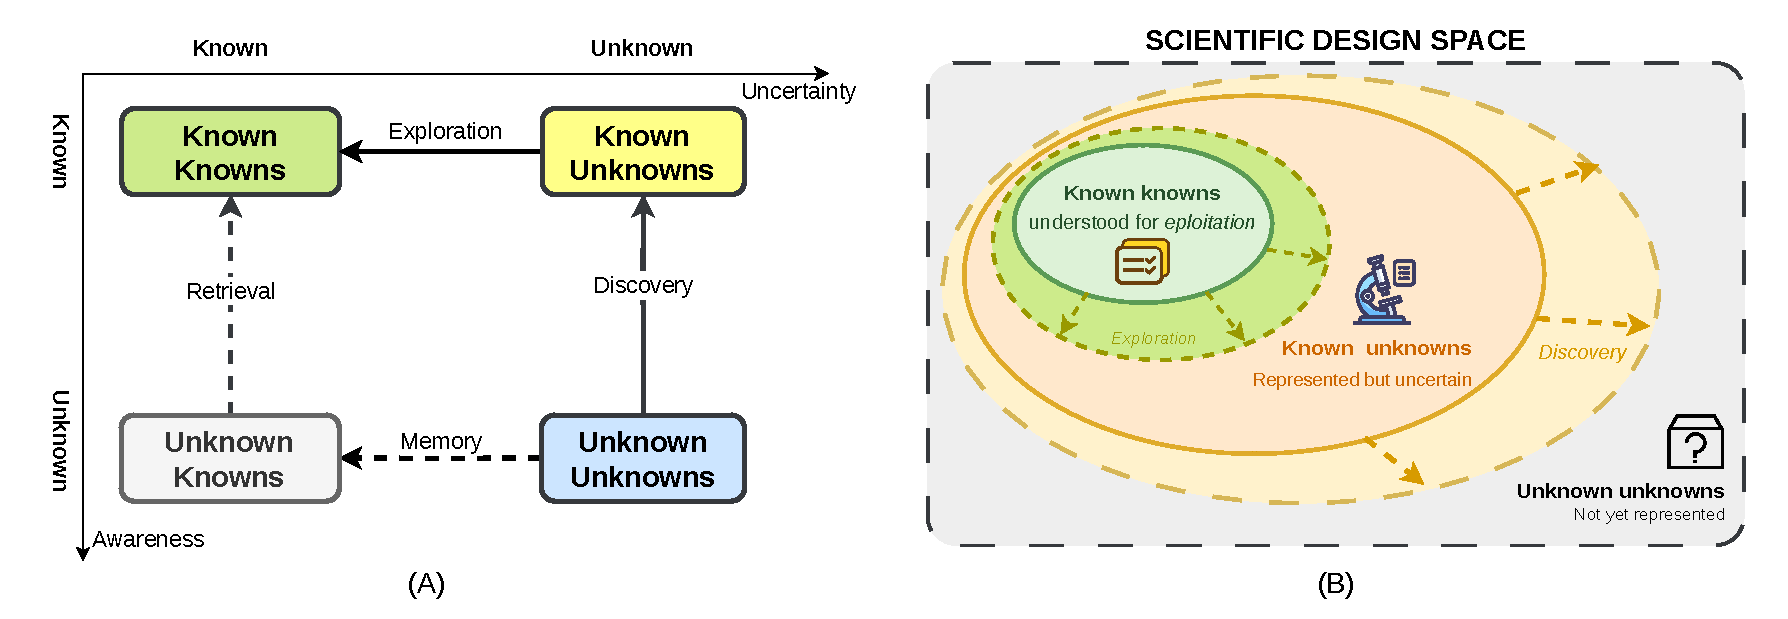
\includegraphics[width=\textwidth]
{figure/scientific_discovery_knowledge_map.drawio.pdf}
    \caption{
    \textbf{Epistemic regimes of experimental scientific search.}
    \textbf{(A)} An adaptation of the Rumsfeld Matrix
\citep{krogerus2018decision}, organised by search awareness and objective
    uncertainty.
    \textbf{(B)} A scientific agent moves among three regimes in the design
    space. 
    %\emph{Discovery} exposes previously unrepresented possibilities and turns them into explicit candidates or research questions. \emph{Exploration} reduces uncertainty about represented candidates and converts them into validated knowledge. \emph{Exploitation} uses this knowledge to select, verify, or deploy promising designs. Unknown knowns, which concern knowledge that is available but not explicitly represented, are outside the scope of this work and are omitted from Panel~B.
    }
    \label{fig:knowledge-regimes}
\end{figure*}

We formalise this problem as \emph{sequential inverse design}. A forward model
predicts the properties of a given design, whereas inverse design asks which
candidate should be evaluated next to achieve a desired property or maximise
an unknown reward. Evaluations may involve physical measurements, simulations,
computational tests, or other external sources of evidence. Because these
evaluations can be costly, only a limited number of candidates can be examined.
At the same time, the structured design space may be combinatorial, effectively
unbounded, or impossible to enumerate. Accurately modelling the reward across
the entire design space is therefore infeasible.

Instead, the agent maintains a \emph{probabilistic surrogate}: a data-efficient
model of the unknown reward learned from the candidates evaluated so far. For
each candidate within its modelling support, the surrogate provides both a
predicted reward and an estimate of \emph{epistemic uncertainty}. Epistemic
uncertainty reflects limitations in the surrogate's knowledge arising from
insufficient or uninformative observations. It can therefore be reduced by
collecting relevant new evidence. This differs from irreducible randomness or
measurement noise in the evaluation itself. After each evaluation, the new
observation is incorporated into the surrogate, updating both its predictions
and its uncertainty.

An \emph{acquisition function} converts the surrogate's predictions and
uncertainties into a measure of how useful it would be to evaluate or further
develop each candidate. It balances candidates predicted to perform well
against candidates that remain uncertain but potentially valuable. An
acquisition value is therefore not simply a predicted reward; it represents
the candidate's value to the sequential search process. The agent uses this
signal to allocate limited inference-time computation and to select candidates
for costly empirical evaluation. It consequently alternates among candidate
generation, evaluation selection, and belief updating.

This formulation separates two epistemic dimensions. The first is
\emph{predictive uncertainty}: how uncertain the surrogate is about the reward
of a candidate represented within its current modelling support. The second is
\emph{search awareness}: whether a candidate is represented by, or reachable
through, the current proposal and search process. Together, these dimensions
distinguish three modes of scientific search:

\begin{itemize}
    \item \emph{Exploitation} selects reachable candidates that the surrogate
    predicts will perform well.

    \item \emph{Exploration} evaluates reachable candidates about which the
    surrogate has high epistemic uncertainty, thereby improving knowledge
    within the current search support.

    \item \emph{Discovery} expands or reshapes the search support to reveal
    candidates, design families, or relationships that were not previously
    represented or reachable.
\end{itemize}

Figure~\ref{fig:knowledge-regimes} illustrates this perspective by adapting
the four epistemic regimes to scientific design. It distinguishes uncertainty
about candidates within the current search support from a lack of awareness of
candidates outside that support. Exploration reduces uncertainty about what is
already represented, whereas discovery changes what can be represented and
reached.

Motivated by this distinction, we introduce the \emph{Large Discovery Model}
(LDM), an empirically grounded recurrent architecture that couples an LLM
proposal model with a continually updated probabilistic surrogate. The LLM
generates, edits, and refines structured candidates, thereby constructing a
dynamic search frontier. The surrogate estimates the candidates' rewards and
quantifies its epistemic uncertainty about them. The acquisition function uses
these estimates to determine which candidates merit further refinement,
additional inference-time computation, or costly empirical evaluation. Each
new observation updates the surrogate and, through the acquisition signal,
redirects subsequent generation and search.

The acquisition function is therefore more than a post-generation filter. It
provides an empirically grounded value signal for allocating both computational
and evaluation resources. The LLM expands and reshapes the set of reachable
candidates, while the surrogate and acquisition function guide search over
this evolving set. In this way, LDM extends inference-time scaling from tasks
with cheap and repeatable verifiers to scientific-design problems
characterised by costly, noisy, and limited empirical feedback.
\begin{figure*}[t]
    \centering
    \begin{subfigure}[t]{0.42\textwidth}
        \centering
        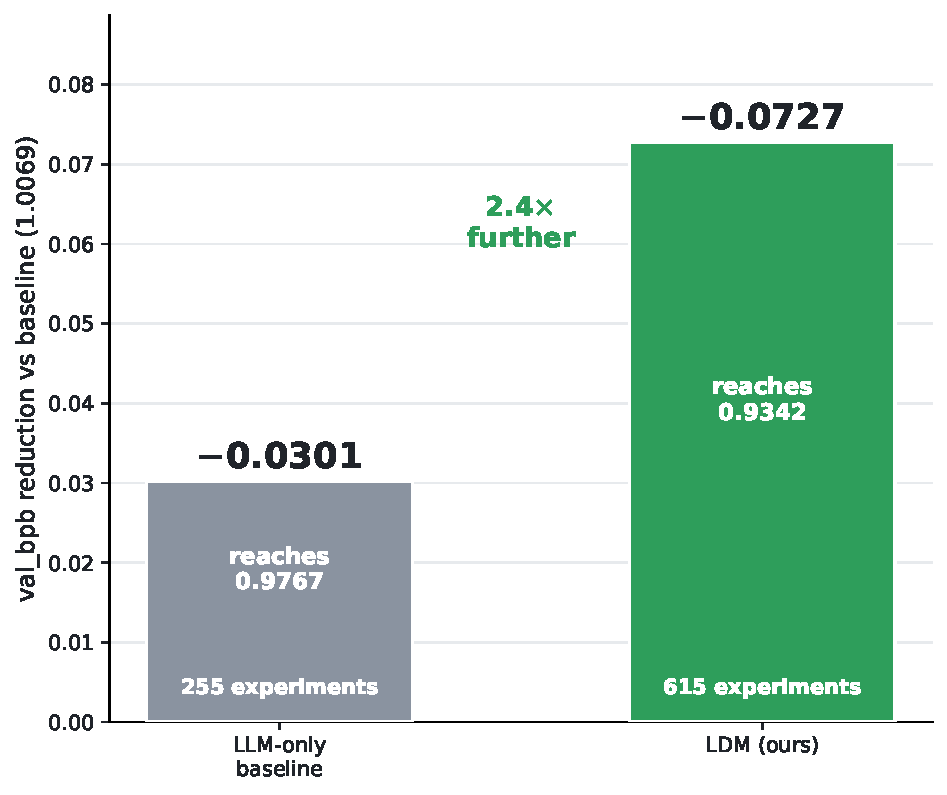
\includegraphics[width=\linewidth]
        {figure/improvement_two_bar.pdf}
        \caption{Performance on AutoResearch.}
        \label{fig:discovery-motivation-autoresearch}
    \end{subfigure}
    \hfill
    \begin{subfigure}[t]{0.42\textwidth}
        \centering
        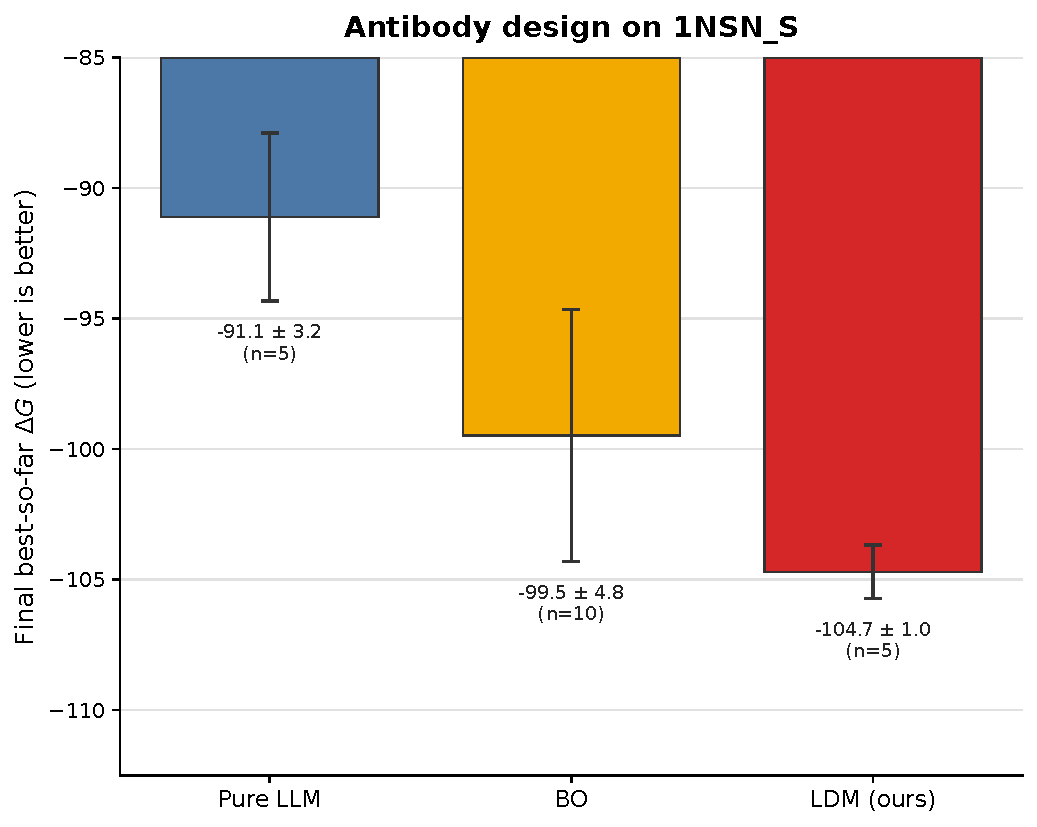
\includegraphics[width=\linewidth]
        {figure/discovery_motivation_antibody_1NSN_S.pdf}
        \caption{Performance on antibody design.}
        \label{fig:discovery-motivation-antibody}
    \end{subfigure}
    \caption{
    \textbf{Complementary limitations of LLM-only and BO-based search.}
    \textbf{(a)} LDM improves upon the LLM-only AutoResearch baseline under
    the same H100 hardware setting.
    \textbf{(b)} Final best-so-far binding energy on the antibody-design task,
    where LDM outperforms the LLM-only and BO-only baselines. Lower binding
    energy is better. For details, we refer to \S~\ref{sec:eval}.
    }
    \label{fig:discovery-motivation}
\end{figure*}


We evaluate LDM in three structured scientific-design domains:
neural-network training-program search on AutoResearch
\citep{karpathy2026autoresearch}, antibody CDRH3 sequence design, and
multi-objective molecular optimisation. LDM exceeds the best previously
reported AutoResearch result. With a weak language-model prior, it remains
competitive with AntBO~\citep{khan2022antbo}, a specialised BO method for
antibody design. It also achieves substantial improvements over both LLM-only
and BO-only baselines in multi-objective molecular design. Figure~\ref{fig:discovery-motivation} presents selected
results, with the full experimental evaluation deferred to
\S~\ref{sec:eval}.

Our contributions are fourfold. First, we formulate scientific discovery as
inference-time search over a dynamic, structured design space, guided by an
uncertainty-aware value model grounded in empirical observations. Second, we
introduce an acquisition-tilted search policy that combines the structured
prior of an LLM with inference-time computation and sequential experimental
feedback. Third, we provide a regret analysis that separates surrogate-model
error from the suboptimality of the LLM-based search process. Finally, we
demonstrate the framework across three classes of scientific objects:
computer programs, biological sequences, and molecules.


The remainder of the paper is organised as follows.
\S~\ref{sec:ldm} introduces the idea of discovery and its epistemic regimes.
\S~\ref{sec:method} derives the LDM formulation and its acquisition-tilted search method. \S~\ref{sec:algo} presents the practical algorithm.
\S~\ref{sec:theory-main} provides the regret analysis.
Finally, \S~\ref{sec:eval} reports the empirical results.

